\documentclass[a4paper,11pt]{memoir}
\usepackage[utf8]{inputenc}
\usepackage[english]{babel}
\usepackage[T1]{fontenc}    
\usepackage[margin=2.5cm]{geometry}
\usepackage{listings,hyperref,color}
\usepackage[final]{pdfpages}
\usepackage{titlesec}

\usepackage{tipa}

\definecolor{lightgray}{rgb}{0.95,0.95,0.95}
\definecolor{lightgreen}{rgb}{0,0.6,0}

\titleformat{\section}
{\normalfont\large\bfseries}
{\thesection\hskip 9pt\textpipe\hskip 9pt}
{0pt}
{}

\titleformat{\chapter}
{\normalfont\Large\bfseries}
{\thechapter\hskip 9pt\textpipe\hskip 9pt}
{0pt}
{}

\lstset{
	frame=tblr,
	keywordstyle=\color{blue}\textbf,
	backgroundcolor=\color{lightgray},
	commentstyle=\color{lightgreen},
	basicstyle=\footnotesize,
	showstringspaces=false,
	tabsize=2
}


\copypagestyle{plainnotice}{plain}
\makeevenhead{plainnotice}{S{\o}ren Hvidberg Frandsen, sfrand12 \\ Troels Beck Kr{\o}gh, tkragh13}{}{Marc Tom Thorgersen, mthorg13 \\ Mathias Sass Michno mmichn13}% not used with "openright"
\makeoddhead{plainnotice}{S{\o}ren Hvidberg Frandsen, sfrand12 \\ Troels Beck Kr{\o}gh, tkragh13}{}{Marc Tom Thorgersen, mthorg13 \\ Mathias Sass Michno mmichn13}% not used with "openright"
\aliaspagestyle{chapter}{plainnotice}


\begin{document}
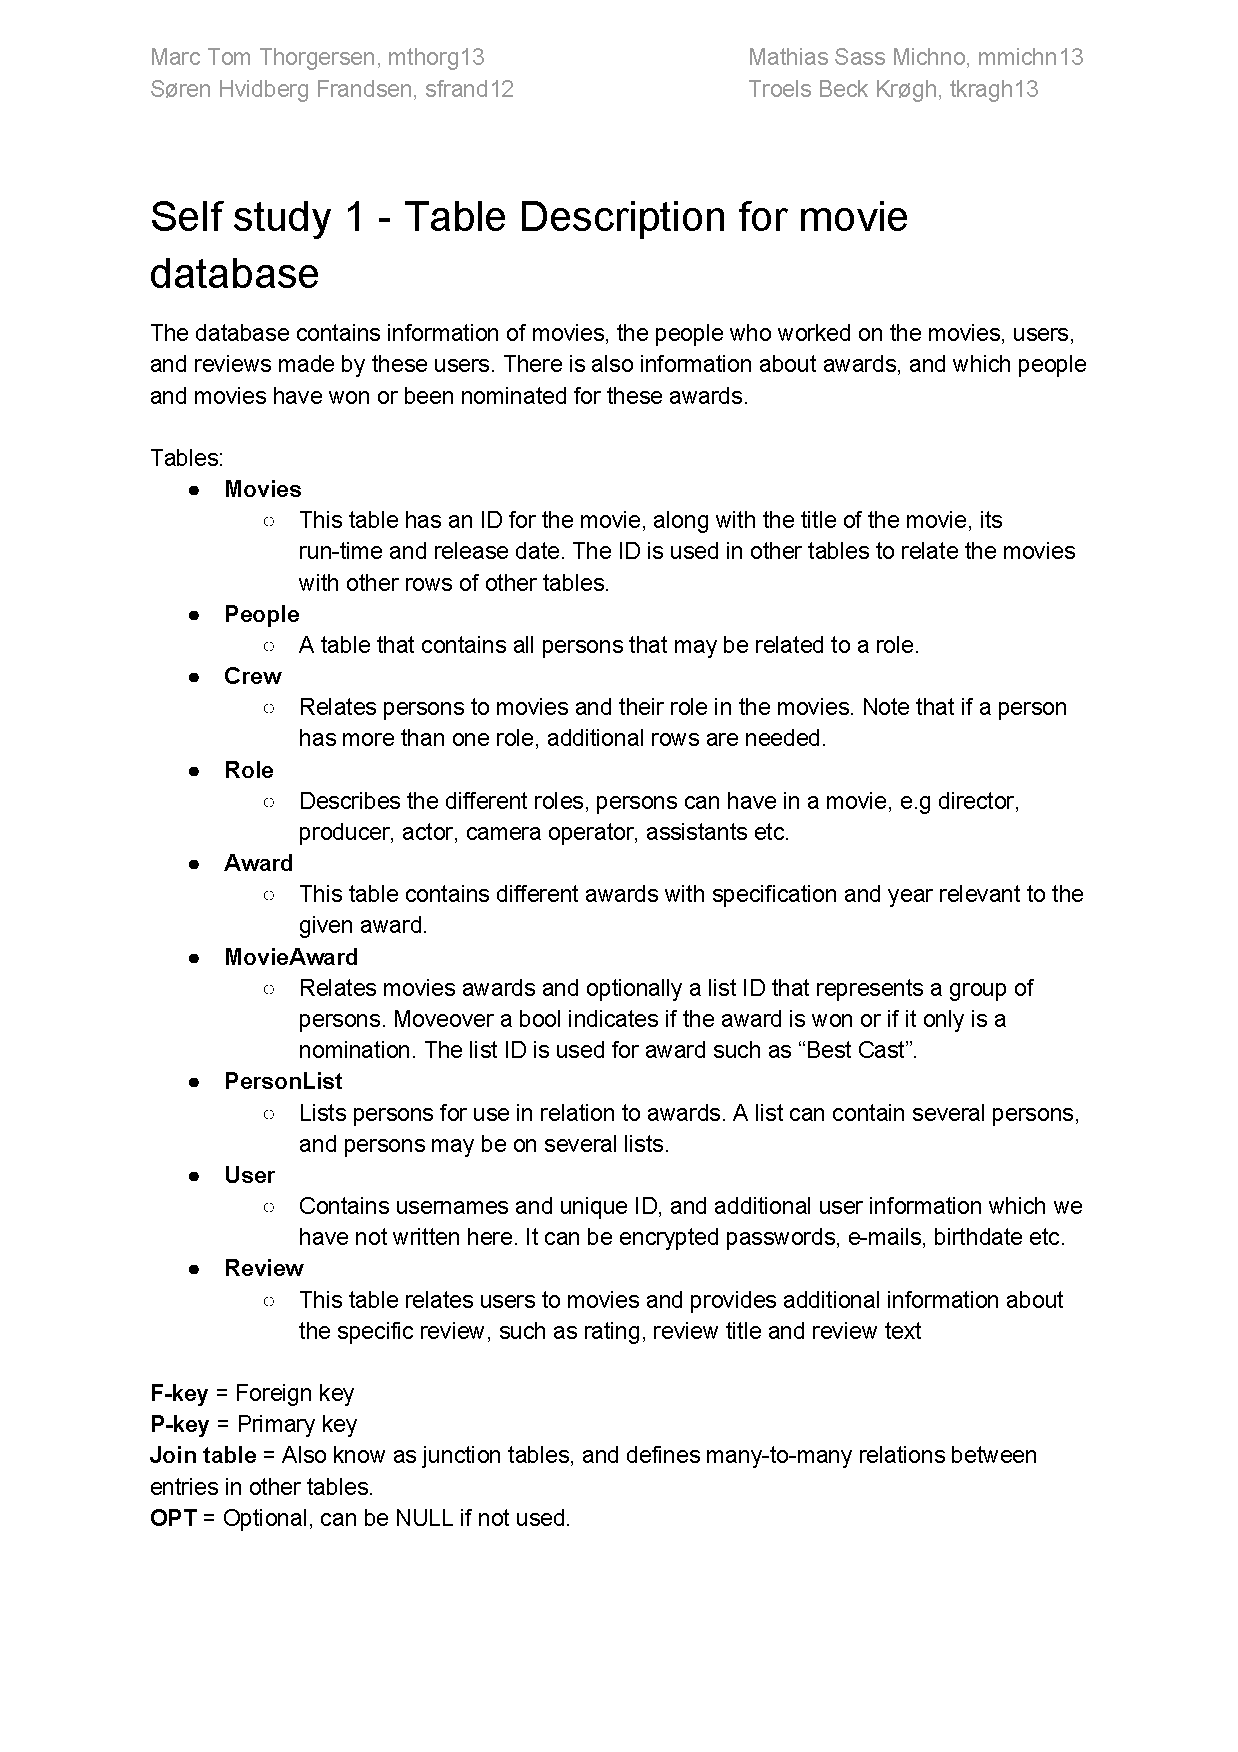
\includepdf[pages=-]{mmichn13mthorg13sfrand12tkragh13.pdf}
\pagestyle{plainnotice}
\part*{Self Study 5}
\chapter{Setting up Postgres}
Install PostgreSQL from \url{http://www.postgresql.org/download/}.
Ensure that the \texttt{pqsl} is in the path of your preferred terminal.
Ensure that PostgreSQL is running by browsing to it in the pgAdmin III tool.
Ensure that PostgreSQL is running on port 5432 by looking in the pgAdmin III tool. 
It might be nesseary to set a enviroment varible with the password: \texttt{export PGPASSWORD=yourpasswordhere}.
Then run the following commands:
\begin{lstlisting}[language=bash]
psql -U postgres -h localhost -p 5432 -c "create database ss"
# OUTPUT:
CREATE DATABASE

psql -U postgres -h localhost -p 5432 -d ss -f schema.sql
# OUTPUT:
REATE TABLE
CREATE TABLE
/* ... */

psql -U postgres -h localhost -p 5432 -d ss -f insert.sql
# OUTPUT:
INSERT 0 251
INSERT 0 58179
/* ... */

\end{lstlisting}

Henceforth the database is ready to use, and should have the appropriate data. 
The database can be queried in the commandline by:
\begin{lstlisting}[language=bash]
# Using a query directly
psql -U postgres -h localhost -p 5432 -d ss -c "select * from movie limit 10;"

# Using a file (query.sql)
psql -U postgres -h localhost -p 5432 -d ss -f query.sql

# Or interactive (NOT RECOMMENDED)
psql -U postgres -h localhost -p 5432 -d ss
\end{lstlisting}
Alternatively the GUI query tool can be used, this is opened though the pgAdmin III tool. 

\chapter{Updates to the database}
\begin{lstlisting}[language=sql]
update person
	set gender='f'
	where id = 666;
\end{lstlisting}
\begin{lstlisting}[language=sql]
update movie
	set title='Calculator Jokes'
	where id = 8008135;
\end{lstlisting}

\chapter{Queries}

\section{How many Danish language movies are in the database?}
\lstinputlisting[language=sql]{sql/1.sql}
\lstinputlisting{sql_res/1.sql}

\section{For each year, what is the total number of reviews to movies from that year?}
\lstinputlisting[language=sql]{sql/2.sql}
\lstinputlisting{sql_res/2.sql}

\section{Which movies have John Travolta and Uma Thurman starred in together?}
\lstinputlisting[language=sql]{sql/3.sql}
\lstinputlisting{sql_res/3.sql}

\section{How many actors and directors have a first name starting with ``Q''?}
\lstinputlisting[language=sql]{sql/4.sql}
\lstinputlisting{sql_res/4.sql}

\section{How many users rated at least 3 movies?}
\lstinputlisting[language=sql]{sql/5.sql}
\lstinputlisting{sql_res/5.sql}

\section{What is the name and birth year of all actors in ``Pulp Fiction''?}
\lstinputlisting[language=sql]{sql/6.sql}
\lstinputlisting{sql_res/6.sql}

\section{What are the titles and years of all movies from the 1980s that John Travolta starred in?}
\lstinputlisting[language=sql]{sql/7.sql}
\lstinputlisting{sql_res/7.sql}

\section{What are the top-2 highest rated movies (average) from the 1990s according to the users?}
\lstinputlisting[language=sql]{sql/8.sql}
\lstinputlisting{sql_res/8.sql}

\section{What are the top-2 highest rated movies (average) from the 1990s according to at least 2 users?}
\lstinputlisting[language=sql]{sql/9.sql}
\lstinputlisting{sql_res/9.sql}

\section{In 1994, what was the average rating of a movie for each language?}
\lstinputlisting[language=sql]{sql/10.sql}
\lstinputlisting{sql_res/10.sql}

\section{Which actors in ``Pulp Fiction'' have never, before or after, starred in the same movie as one of the other actors in ``Pulp Fiction''?}
\lstinputlisting[language=sql]{sql/11.sql}
\lstinputlisting{sql_res/11.sql}

\section{Which movie starring John Travolta has the highest user ratings?}
\lstinputlisting[language=sql]{sql/12.sql}
\lstinputlisting{sql_res/12.sql}

\section{How many actresses have not been alive at the same time as Charles Chaplin?}
\lstinputlisting[language=sql]{sql/13.sql}
\lstinputlisting{sql_res/13.sql}

\section{What is the average rating of movies from each genre?}
\lstinputlisting[language=sql]{sql/14.sql}
\lstinputlisting{sql_res/14.sql}

\section{What is the average rating of movies from each genre? List only genres with at least 2 ratings.}
\lstinputlisting[language=sql]{sql/15.sql}
\lstinputlisting{sql_res/15.sql}

\section{Which movie has the largest number of 2-link references?}
\lstinputlisting[language=sql]{sql/16_2.sql}
\lstinputlisting{sql_res/16.sql}

\section{How many actors have also been active as director of at least one movie?}
\lstinputlisting[language=sql]{sql/17_2.sql}
\lstinputlisting{sql_res/17.sql}


\section{Which two genres are most often linked to the same movie? (Note that each movie has a set of genres.)}
\lstinputlisting[language=sql]{sql/18.sql}
\lstinputlisting{sql_res/18.sql}


\end{document}